\documentclass[12pt]{article}
\usepackage{amsmath}
\usepackage{graphicx}
\DeclareGraphicsExtensions{.pdf,.png,.jpg}

\newtheorem{theorem}{Theorem}[section]
\newtheorem{lemma}[theorem]{Lemma}
\newtheorem{definition}[theorem]{Definition}


\title{Covering CSpace}
\date{}
\begin{document}
  \maketitle
  \section{Model}
	Define an estimate cost function for diff drive or R.S car as:

  $C( d, \theta ) = f(d) + g(\theta)$

  where $d$ is the euclidean distance from start to goal and $\theta$ is the different of orientation. \\

  $f(d) = k(d) * d$ is a monotonically decreasing function.

  $g(\theta) \in [0, \pi]$

  \section{Outer Circle and Inner Circle}
  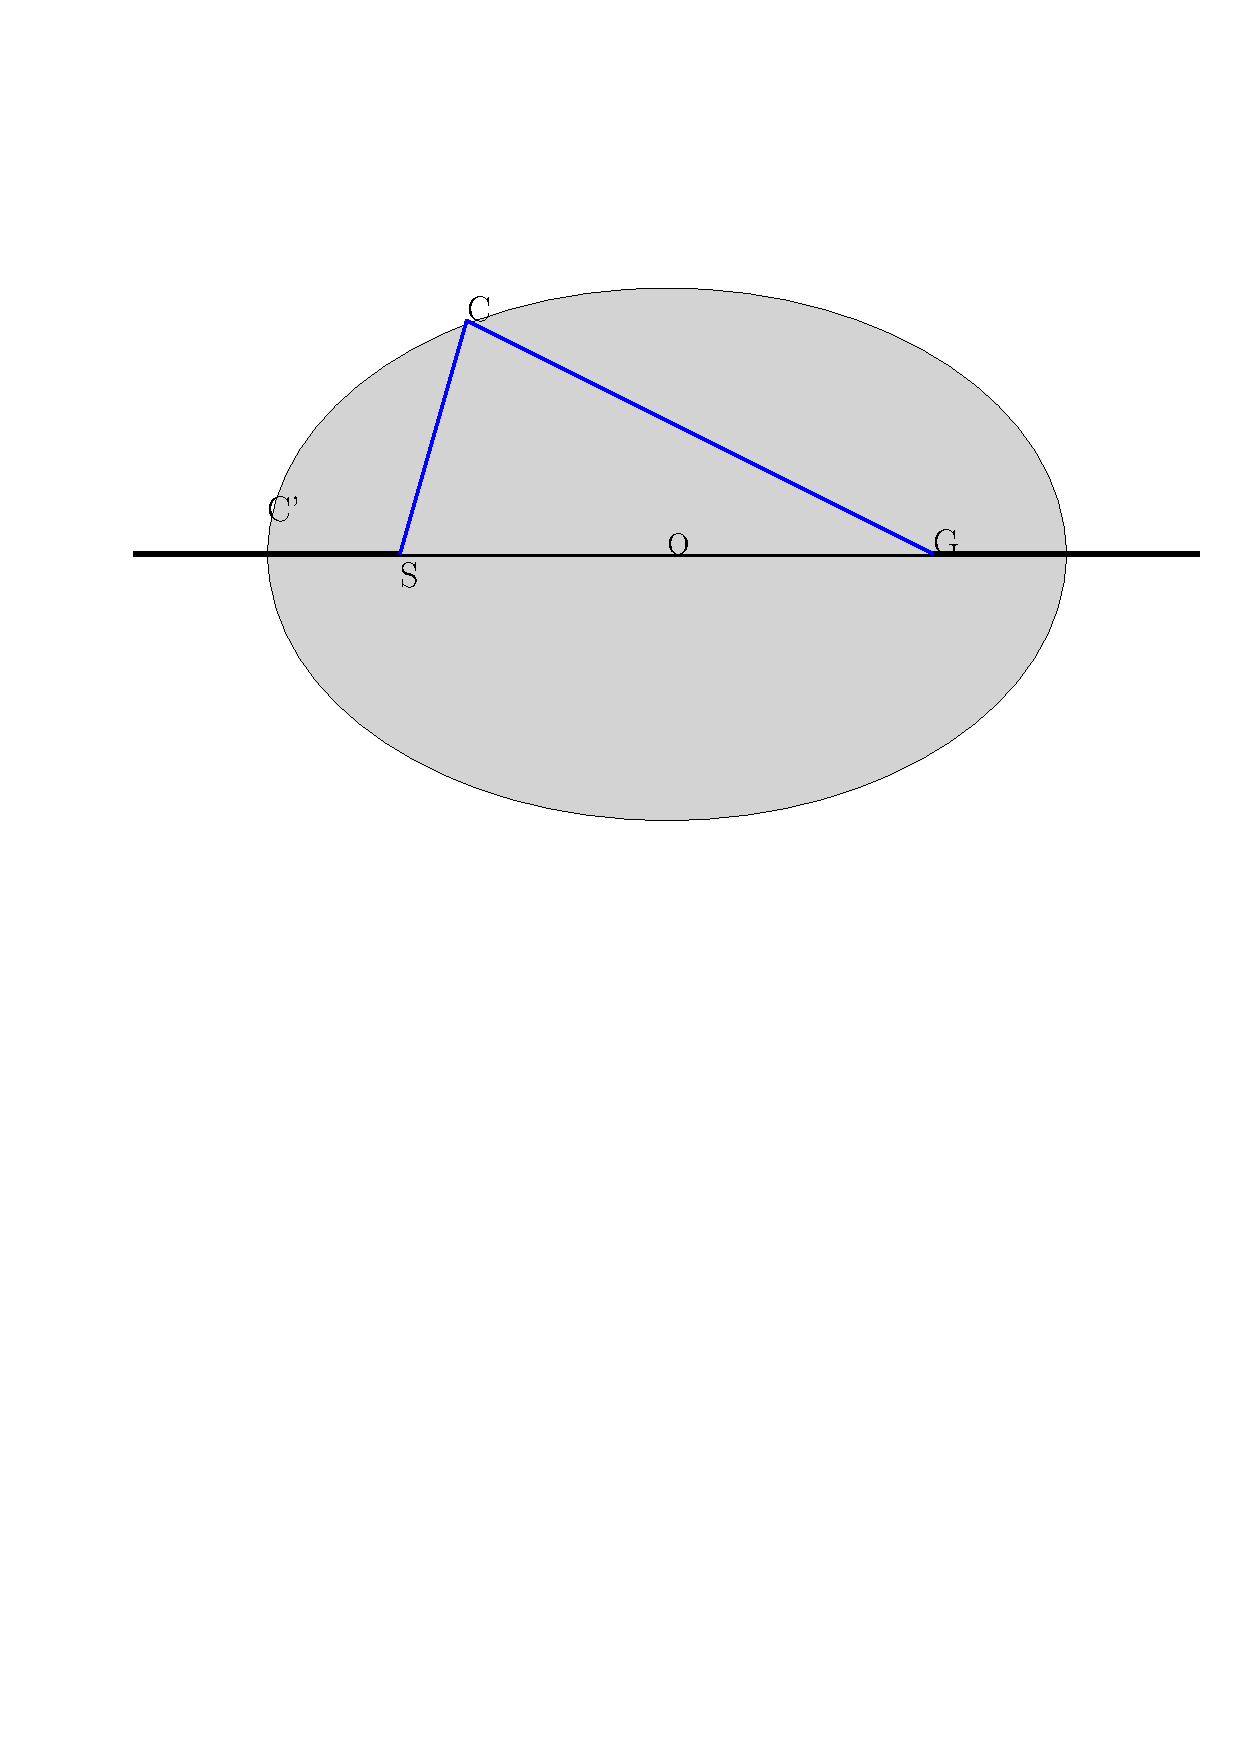
\includegraphics[scale=0.7]{Ellipse}\\

  Assume $C$ being a point in the workspae and $|SC|+|GC| \leq C( d, \theta )$. C is in an ellipse with foci's S and G. \\ 
  
  Since any point P out side the ellipse will have $|SP| + |PG| > C( d, \theta )$, the optimal path from S to G with any orientation must be within the ellipse.\\
  
  $C'$ is a intersect point of line $SG$ and the ellipse. $O$ is the mid point of S and G. \\
  
  $\Longrightarrow$ $|SO| = |OG| = \frac{d}{2}$. $|C'S| + |C'G| = C( d, \theta ) = 2|C'S| + |SG|$
  
  $\Longrightarrow$ $|C'S| = \frac{C( d, \theta )}{2} - \frac{d}{2}$

  $\Longrightarrow$ $|C'O| = |C'S|+|SO| = \frac{C( d, \theta )}{2} - \frac{d}{2} + \frac{d}{2} = \frac{C( d, \theta )}{2}$\\

  By rotating S and G about their mid point O, the trajectory of C' is the edge if another ball with radius $\frac{d}{2} + \frac{C( d, \theta )}{2}$. And between any points in the inner ball with $\theta$ difference of orientation, there must exist an optimal trajectory without leaving the outer ball. \\

  Define the radius of outer circle as $R$, radius of inner circle as $r$\\

  $\Longrightarrow$ $\frac{|C'O|}{|SO|} = \frac{R}{r} = \frac{C(2r,\theta)}{2} / \frac{d}{2} = \frac{C(2r,\theta)}{d}$\\

  $\Longrightarrow$ $\frac{R}{r} = \frac{C(2r,\theta)}{2r} = \frac{k(2r)*2r + g(\theta)}{2r} = k(2r) + \frac{g(\theta)}{2r}$\\

  \section{From one config to another in a circle}

  Inside a circle with radius $r'$, if we want to move from one config to another with any orientations ( meaning $g(\theta)$ should have the largest value, $g(\theta) = \pi$ ), we need an outer circle with radius $R'$:\\

  $R' = r' * k(2r) + \frac{\pi}{2}$\\

  However, outside the r'-circle, there might not have enough clearance. Assume the center of the r'-circle has R clearance, where $R \leq R' $, if we still want to move from on config to another, we have to reduce some orientation difference to compensate $R-R'$.

  $\Longrightarrow$ $g(\theta) = \pi - (R'-R)$ \\

  \section{From one config to aonther}

  Assume a path has $\delta$ clearance, and a chain of circles totally covers the path. Each two neighbor circles have at least one intersection point. The max radius of these circles is r. ($\delta > r$). $\delta$ is small. By "small", I mean:\\

  $\delta \leq r*k(2r) + \frac{\pi}{2}$\\.

  Therefore, in each circle of the circle chain that covers the path, the cost in changing the orientation can be at most:\\

  $g(\theta) = \pi - ( r*k(2r) + \frac{\pi}{2} - \delta)$.\\

  Suppose in i-th circle, the change of orientation is $\theta_{i}$. There is always a N such that:\\

  $\sum\limits_{i = 1}^N g(\theta_{i}) \geq \theta_{needed}$\\
  
  This means that if we can't make a turn that costs $\theta_{needed}$, we can go in and out the circle for several times.

  \section{Covering the narrow passage in c-space}

  ( If you are reading from here, previous sections are saying that for an inner circle, we might not have the clearance that allows an optimal path connecting any two configurations with any orientation. Therefore, to reach from one point to another, we have to change less of orientations. But a chain of circles can still cover a path. )\\

  The conclusion from last section is suggesting that, for a narrow passage with max of clearance $\delta$ in any point, we can have a chain of r-circles ( $r < \delta$ ) such that for a start configuration at the head of the chain and a goal configuration at the end, there is a path that is collision free.\\

  (Wait a moment... is the path optimal? It seems we could only estimate the cost of the path. Hmm... I should think about that.)\\

  In C-space, these circles are cylinders that constrain some orientation change in each cylinder. They are kind of stairs in C-space, and these stairs covers the optimal (optimal???) path in C-Space. \\
  
  \hspace*{-2cm}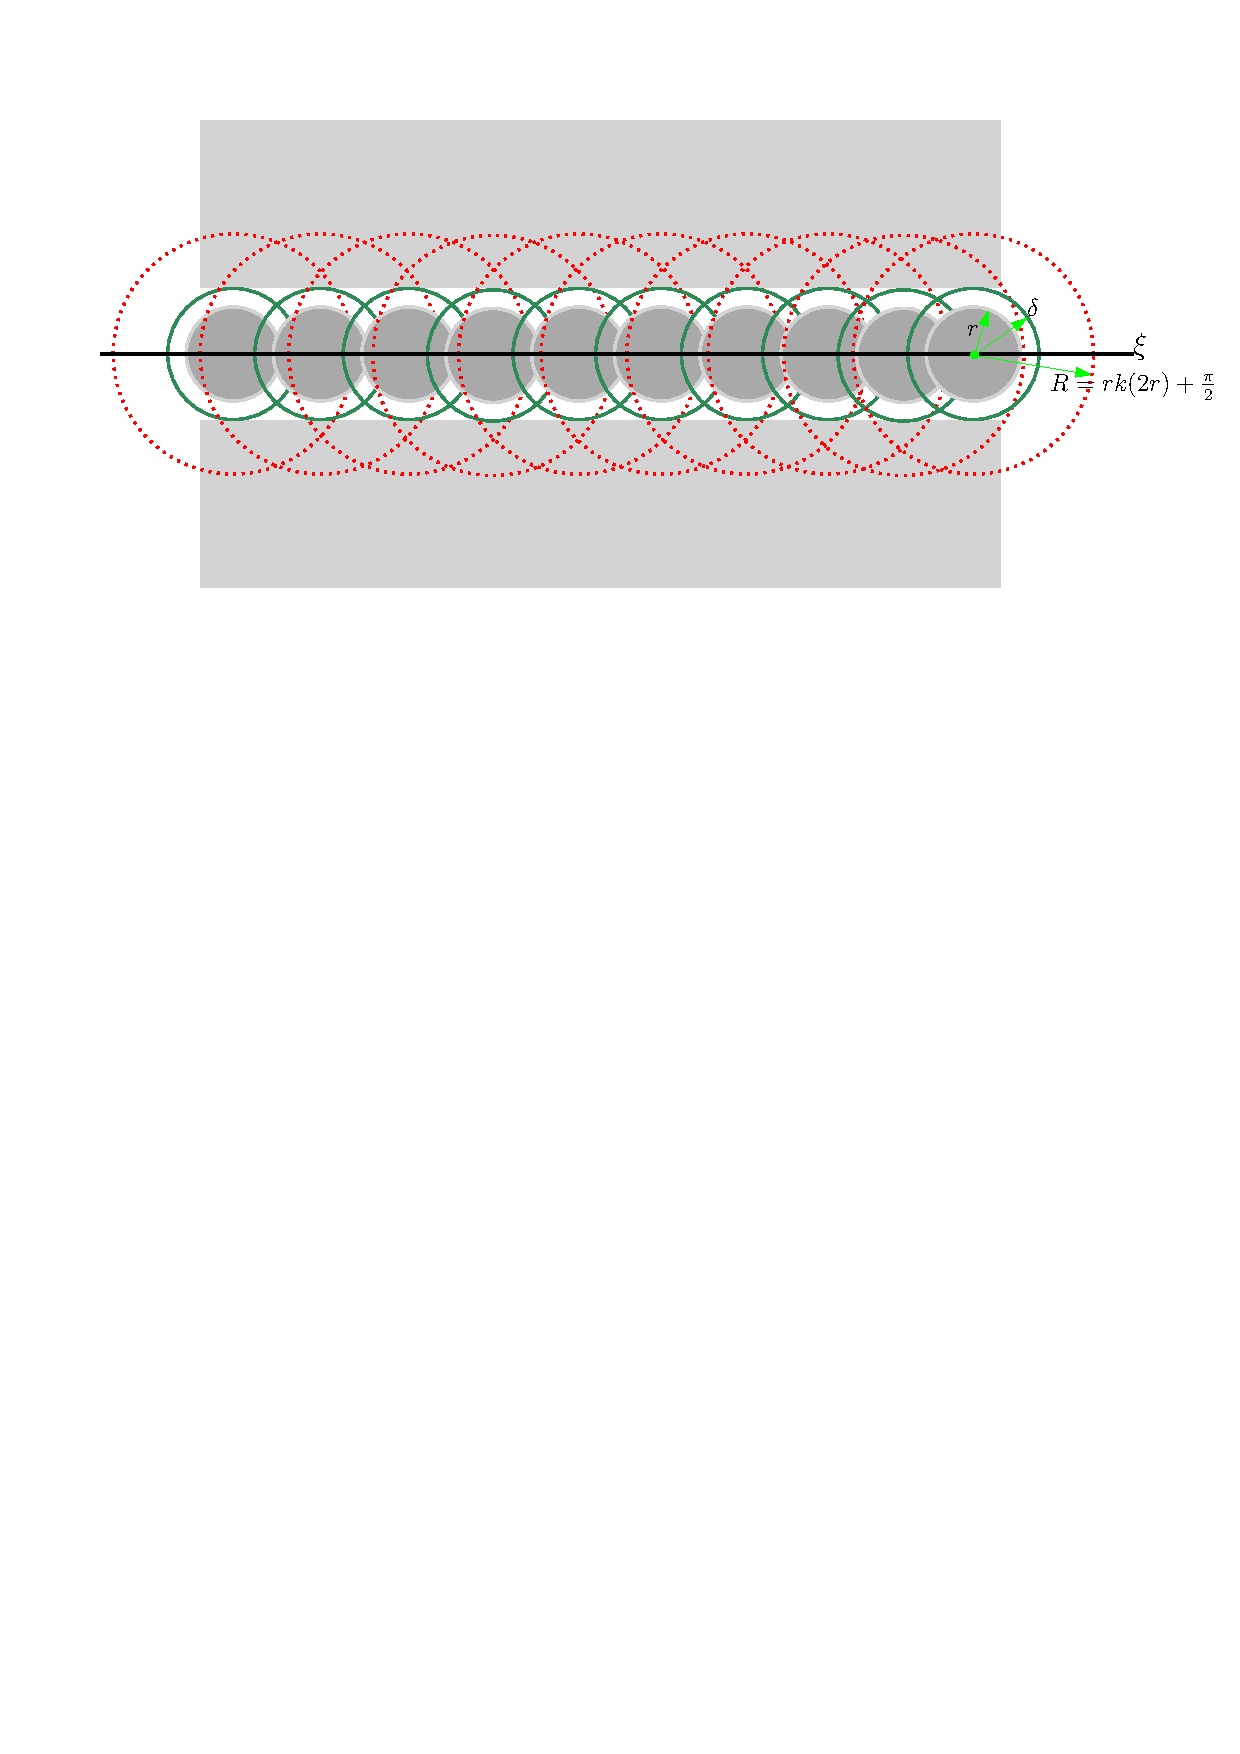
\includegraphics[scale=0.84]{CirclesCoveredPath}\\

  In a narrow passage with $\delta$ clearance.( $\delta<\pi / 2$ ) If we are covering the space with circles of radius $r = \frac{\delta}{n}$:\\
  
  $g(\theta) = \pi - (r*k(2r) + \frac{\pi}{2} - \delta) = \pi - ( \frac{f(\frac{2\delta}{n})}{2} + \frac{\pi}{2} - \delta )$,\\
  
  $\frac{\pi}{2} - \delta \in (0, \frac{\pi}{2})$\\
  
  we want $\frac{f(\frac{2\delta}{n})}{2} \in (0, \frac{\pi}{2})$\\
  
  $\Longrightarrow$ $f(\frac{2\delta}{n}) \in (0, \pi)$\\
  
  n tends to be large. But we probably can find a heuristic n such that n is not too large, then we don't need too large clearance for an optimal path, nor too small, so we can get more close to obstacles.
  
  \section{Dealing with a big turn in a small circle }
  
  Sometimes you have to make a big turn in a small circle. As implied at the end of section 4, we can do it by leaving and entering the same circle several times. For diff drive, we can simply make the turn without moving. For RS car, we need to decide what are the points we leave and enter the circle.\\
  
  (To be continued....)
  
  \section{Estimating the cost of generated path and optimal path}
  
  (To be continued....)

\end{document}